\section{Agentic UI and Web Generation}
\label{sec:ui-web}

Interface generation joins visual appearance to executable behavior. Component trees, style rules, screenshots, browser state, and interaction traces provide complementary views of the same artifact, making this domain a stringent test of whether visual feedback can be translated into code-level repair.

\begin{keytakeaway}[Agentic UI and Web Generation at a Glance]
\begin{keypoints}
  \item \textbf{From visual specification to executable interface:} coordinate design intent with component structure and runtime behavior, treating a rendered screenshot as an observation of the program rather than a substitute for functional state.

  \item \textbf{Browser-grounded verification and repair:} combine screenshots, DOM structure, interaction tests, and accessibility checks, where this heterogeneous evidence makes precise repair possible but also reveals failures that a single image metric cannot capture.
\end{keypoints}
\end{keytakeaway}

\begin{figure}[!htbp]
  \centering
  
\definecolor{avgmapblue}{HTML}{22558A}
\definecolor{avgmapgreen}{HTML}{23845D}
\ifdefined\avgmapfont\else\newcommand{\avgmapfont}{\rmfamily}\fi
\makebox[\linewidth][c]{%
\resizebox{0.98\linewidth}{!}{%
\begin{tikzpicture}[
  avg branch/.style={draw=avgmapblue!58, fill=avgmapblue!9, text=black!88, rounded corners=2.5pt, line width=0.48pt, text width=42mm, minimum height=10.5mm, align=center, inner xsep=2.2mm, inner ysep=0.9mm, outer sep=0pt, execute at begin node={\hyphenpenalty=10000\exhyphenpenalty=10000\relax}, font=\avgmapfont\fontsize{7.35}{8.35}\selectfont\bfseries},
  avg papers/.style={draw=avgmapblue!25, fill=avgmapblue!2, text=black!88, rounded corners=2.5pt, line width=0.38pt, text width=115mm, minimum height=10.5mm, align=left, inner xsep=3mm, inner ysep=0.9mm, outer sep=0pt, execute at begin node={\hyphenpenalty=10000\exhyphenpenalty=10000\relax}, font=\avgmapfont\fontsize{7.15}{8.25}\selectfont\bfseries},
  avg benchmark branch/.style={avg branch, draw=avgmapgreen!78, fill=avgmapgreen!15, text=avgmapgreen!45!black},
  avg benchmark papers/.style={avg papers, draw=avgmapgreen!72, fill=avgmapgreen!7, text=black!88},
  avg root/.style={draw=avgmapblue, fill=avgmapblue!94!black, text=white, rounded corners=2.5pt, line width=0.55pt, minimum width=9mm, minimum height=36mm, inner sep=0pt, outer sep=0pt},
  avg line/.style={draw=black!28, line width=0.45pt, line cap=round},
  avg benchmark line/.style={draw=avgmapgreen!78, line width=0.55pt, line cap=round}
]
\matrix (avgmap) [matrix of nodes, row sep=1.35mm, column sep=3mm, ampersand replacement=\&, nodes={anchor=center}] {
  \node[avg branch] (c9b1) {Executable Interfaces}; \& \node[avg papers] (c9p1) {MM-WebAgent~\cite{avg260415309}, MAxPrototyper~\cite{yuan2024maxprototyper}, GameUIAgent~\cite{avg260314724}.}; \\
  \node[avg branch] (c9b2) {Browser-Grounded Repair}; \& \node[avg papers] (c9p2) {Replit Agent~\cite{replit2024agent}, Bolt.new~\cite{stackblitz2024boltnew}, Lovable~\cite{lovable2024docs}, PlayCoder~\cite{avg260419742}, TDDev~\cite{avg250925297}.}; \\
  \node[avg benchmark branch] (c9b3) {Benchmarks}; \& \node[avg benchmark papers] (c9p3) {VISTA~\cite{avg260526144}, Vision2Web~\cite{avg260326648}.}; \\
};
\coordinate (c9trunktop) at ($(c9b1.west)+(-4.6mm,0)$);
\coordinate (c9trunkbottom) at ($(c9b3.west)+(-4.6mm,0)$);
\coordinate (c9rootnw) at ($(c9b1.north west)+(-15.5mm,0)$);
\coordinate (c9rootse) at ($(c9b3.south west)+(-7.6mm,0)$);
\node[avg root, fit=(c9rootnw)(c9rootse)] (c9root) {};
\node[rotate=90, align=center, text=white, font=\avgmapfont\fontsize{7.05}{8.15}\selectfont] at (c9root.center) {{\bfseries CHAPTER 9}\\[0.55mm]{\fontsize{6.2}{7.15}\selectfont UI and Web generation}};
\draw[avg line] (c9trunktop) -- (c9trunkbottom);
\coordinate (c9trunkmid) at ($(c9trunktop)!0.5!(c9trunkbottom)$);
\draw[avg line] (c9root.east) -- (c9trunkmid);
\draw[avg line] (c9trunktop |- c9b1.west) -- (c9b1.west);
\draw[avg line] (c9b1.east) -- (c9p1.west);
\draw[avg line] (c9trunktop |- c9b2.west) -- (c9b2.west);
\draw[avg line] (c9b2.east) -- (c9p2.west);
\draw[avg benchmark line] (c9trunktop |- c9b3.west) -- (c9b3.west);
\draw[avg benchmark line] (c9b3.east) -- (c9p3.west);
\end{tikzpicture}%
}%
}

  \caption{Representative systems and benchmarks for agentic UI and Web generation, organized according to the chapter taxonomy.}
  \label{fig:ch9-representative-systems}
\end{figure}

\subsection{From visual specification to executable interface.}
Visual-to-code and specification-to-interface systems must coordinate design intent with component structure and runtime behavior. A rendered screenshot is an observation of the program, not a substitute for functional state.

\paragraph{MM-WebAgent}
 is a hierarchical multimodal framework that generates coherent webpages with images, videos, and charts from natural language. It operates through global layout planning, local element planning, parallel AIGC-based generation, and three-tier iterative refinement (local asset, surrounding code, and full page) guided by rendered screenshots~\cite{avg260415309}. Figure~\ref{fig:ch9-mm-webagent-examples} presents representative outputs across several multimodal webpage tasks.

\begin{figure}[!htbp]
  \centering
  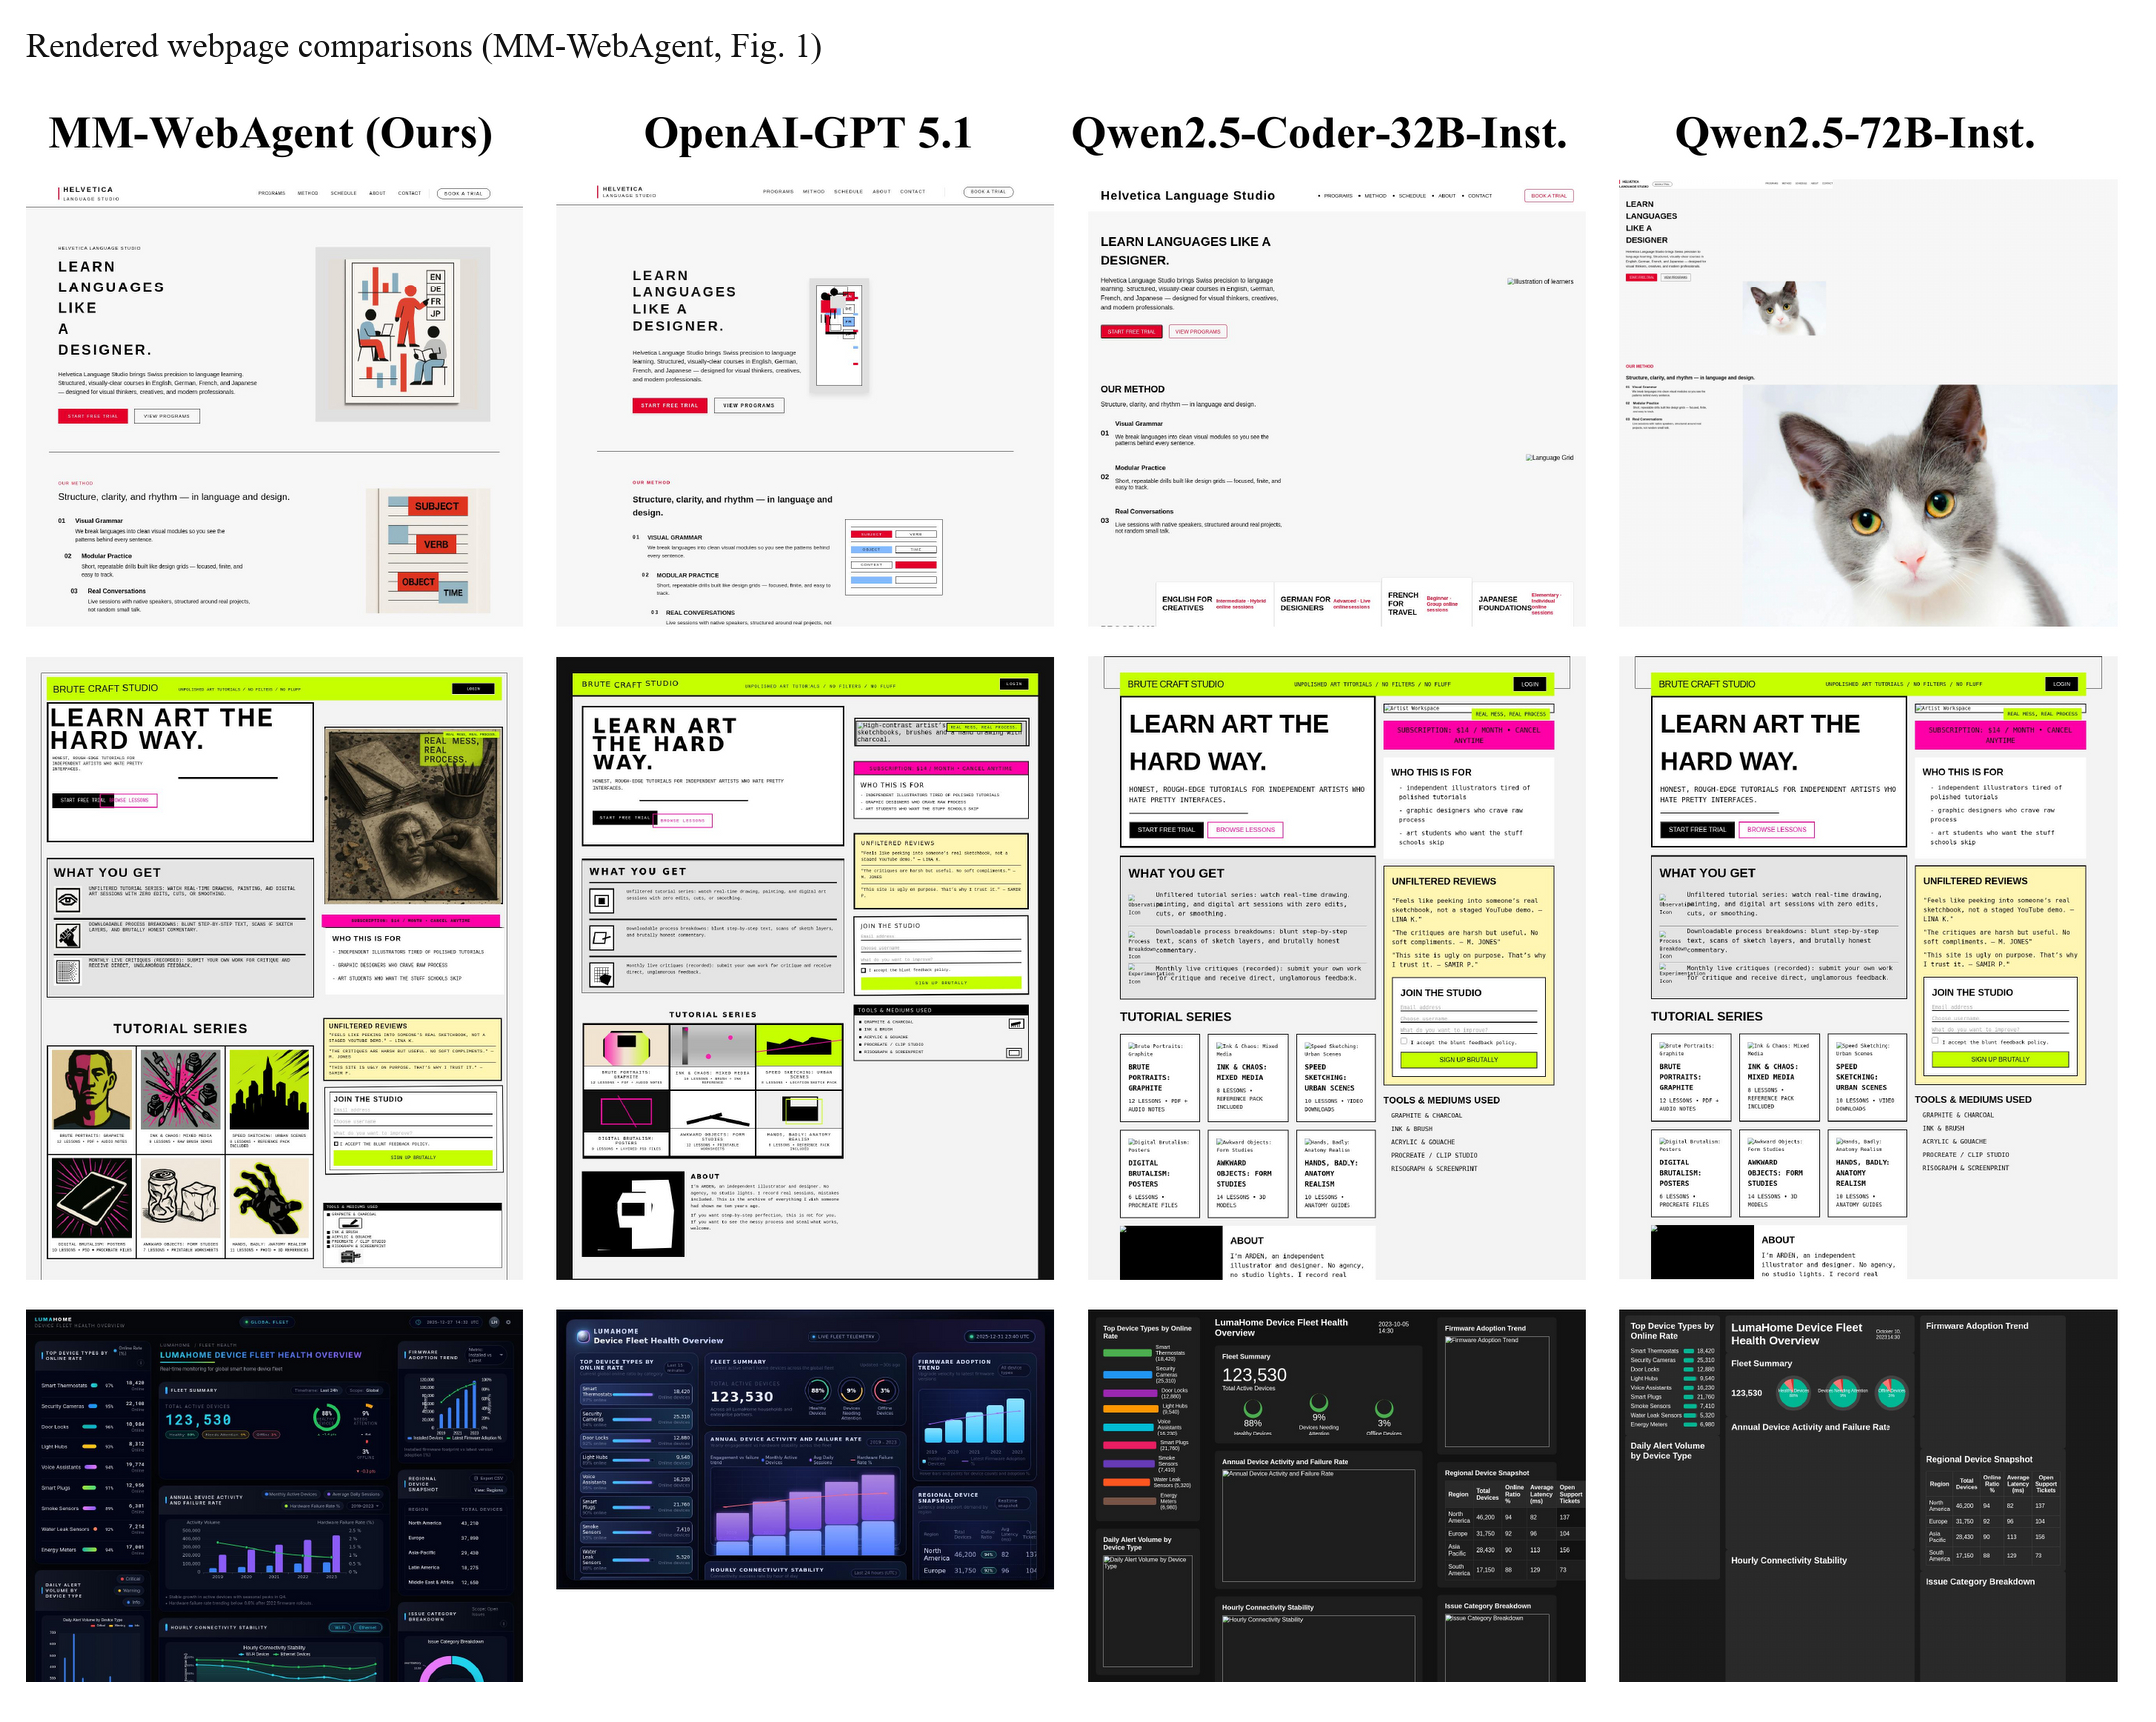
\includegraphics[width=\textwidth]{figures/ch9_multi_agent_ui_prototyping.jpg}
  \caption{Rendered webpage examples generated by MM-WebAgent and representative baselines. Across language-learning, art-tutorial, and device-monitoring pages, the comparison exposes differences in layout completeness, visual-style consistency, and the integration of images, charts, and other multimodal elements~\cite{avg260415309}.}
  \label{fig:ch9-mm-webagent-examples}
\end{figure}

\paragraph{MAxPrototyper}
 is a multi-agent system that converts a text description and a wireframe into an editable UI prototype. A Theme Design Agent sets the global theme and generates a theme image via fine-tuned diffusion with ControlNet, while text, image, and icon agents create each component under its direction, using a cache pool to maintain design context.~\cite{yuan2024maxprototyper}.

\paragraph{GameUIAgent}
 is an LLM-powered framework that generates editable Figma game UI designs from natural language via a Design Spec JSON intermediate representation, combining LLM generation, deterministic post-processing, and a VLM-driven Reflection Controller that iteratively refines designs with guaranteed non-regressive quality~\cite{avg260314724}. The Quality Ceiling Effect (r = -0.96) and Rendering-Evaluation Fidelity Principle further reveal that improvement is bounded by evaluator headroom and that incomplete rendering can paradoxically degrade VLM scores.

\subsection{Browser-grounded verification and repair.}
Browser-grounded systems can combine screenshots, DOM structure, interaction tests, and accessibility checks. This heterogeneous evidence makes precise repair possible but also reveals failures that a single image metric cannot capture.

\paragraph{Replit Agent} is a commercial software-building agent that turns a natural-language application description into a deployed web application: it plans the project as an ordered task list, configures the environment, installs dependencies, writes code, and executes the result, testing its own work and fixing detected problems, while checkpoints preserve intermediate states for rollback~\cite{replit2024agent}. Task-level intent and acceptance remain with the user through chat, but the build--execute--repair loop is driven by runtime evidence rather than by re-prompting.

\paragraph{Bolt.new} runs full-stack application generation entirely in the browser: the model is given complete control over a WebContainers-based environment---filesystem, Node.js server, package manager, terminal, and browser console---so that prompting, running, editing, and deploying happen within a single session~\cite{stackblitz2024boltnew}. Runtime instrumentation captures execution errors and returns them to the model, which automatically tests, refactors, and iterates, though evidence for this loop remains vendor-reported rather than independently benchmarked.

\paragraph{Lovable} is a chat-driven web-application builder whose agent observes build errors, scans project logs and console output, and tests the generated application in a browser to attempt repairs~\cite{lovable2024docs}. A scheduled monitoring mode extends the loop beyond user-initiated turns by watching the deployed project and proposing fixes when issues are detected.


\paragraph{PlayCoder}
 is a multi-agent framework that generates executable GUI application code through a closed-loop of repository-aware generation, automated visual testing, and iterative repair, targeting silent behavioral failures that evade compilation and unit tests~\cite{avg260419742}. 

\paragraph{TDDev}
 is a test-driven development framework that generates full-stack web applications from natural language and optional design images via three agents: test generation, development, and testing (with BrowserUse for interaction simulation), iteratively refining code until all test cases pass~\cite{avg250925297}.

\paragraph{VISTA}
 is a benchmark evaluating end-to-end web-app coding agents under five input conditions varying visual/structural fidelity and stack constraint, with 3,253 annotated interactions across 128 pages~\cite{avg260526144}. It combines DOM-grounded behavior checks with CLIP-based visual similarity. Among four model–harness systems, free-stack conditions yield the best Combined scores (~0.26). Opus achieves the highest Combined (0.261) and behavior (0.336), while GPT-5.5 attains the best CLIP (0.853) but lowest behavior (0.283), revealing a decoupling between visual reproduction and functional correctness.

\paragraph{Vision2Web}
 is a hierarchical benchmark for evaluating multimodal coding agents on visual website development across three levels—static, interactive frontend, and full-stack—with 193 tasks, 918 prototypes, and 1,255 test cases~\cite{avg260326648}. It employs workflow-based verification: a GUI agent checks functionality and a VLM judge assesses visual fidelity. Claude Opus 4.5 performs best overall under OpenHands (full-stack VS/FS: 38.4/57.6), while Gemini-3-Pro-Preview leads on static desktop (63.3) but collapses on full-stack (VS 11.7, FS 22.6). The GUI verifier achieves 87.2\% node-level agreement with human annotations, and the VLM judge attains a mean Spearman correlation of 0.66.

UI and Web work provides the clearest opportunity to connect perception to executable repair because the same artifact can be inspected as pixels, a component tree, and runtime behavior. The principal challenge is to preserve this correspondence across long editing trajectories rather than optimizing isolated screenshots.

\FloatBarrier

\Needspace{0.80\textheight}
